\section{Introduction To Distributed Systems (Hadoop as as example)}

%%%%%%%%%%%%%%%%%%%%%%%%%%%%%%%%%%%%%%%%%%%%%%%%%%%%%%%%%%%%%%%%%%%%%%%%%%%%%%%%%%%%%%%%%

\begin{frame}
\frametitle{Chapter Objectives}

\begin{itemize}
	\item<1-> What is data management? \pause
	\item<2-> Introduction to distributed systems concepts \pause
	\item<3-> Why we need Hadoop? \pause
	\item<4-> Understand the concept of HDFS and Map-Reduce.
	\item<5-> Developing Map-Reduce applications. \pause
	\item<5-> Using Hive QL over Map-Reduce. \pause
	\item<7-> Hadoop advantages and disadvantages with use cases? \pause
\end{itemize}

\end{frame}

%%%%%%%%%%%%%%%%%%%%%%%%%%%%%%%%%%%

\subsection{Data Management}

\begin{frame}
\frametitle{Data Management}

\begin{itemize}
	\item Data are a product.
	\item Data product has a life-cycle as following (simplified): 
	\begin{itemize}
		\item \textbf{Question}, Idea, or service.
		\item \textbf{Identifying} the source of information and the data type ex: (text, images, videos, audio, or sensors).
		\item \textbf{Document} all details regarding the data including quality, security, efficiency, and access (consideration during the cycle).
		\item Delivery automation (Tools and Process) AKA \textbf{DevOps} cycle.
		\item \textbf{Extraction} Process (collection).
		\item \textbf{Transformation} ex: (cleansing, Apply business logic, Organize).
		\item \textbf{Loading} or store the transformed data based on our usage or use case.
		\item Business Intelligence (\textbf{BI}) or data discovery (continues process).
		\item \textbf{Integration} and publishing.
		\item Data retention or \textbf{archiving} process ex: (Hot or Cold storage).
	\end{itemize}
\end{itemize}

\end{frame}

%%%%%%%%%%%%%%%%%%%%%%%%%%%%%%%%%%%%%%%%%%%%%%%%%%%%%%%%%%%%%%%%%%%%%%%%%%%%%%%%%%%%%%%%%

\begin{frame}
\frametitle{Data Management Life-Cycle}
\begin{center}			
			\smartdiagramset{circular distance=3.5cm,
				font=\scriptsize,
%				text width=1cm,
				module minimum width=2cm,
				circular distance =3.4cm,
				module minimum height=.1cm,
				arrow tip=to}
			\smartdiagram[circular diagram]{Archiving,Idea, Identify, Document, 				
				 DevOps,Extraction, Loading, BI, Integration}


\end{center}

\end{frame}

%%%%%%%%%%%%%%%%%%%%%%%%%%%%%%%%%%%%%%%%%%%%%%%%%%%%%%


\subsection{From DWH to Big Data}
\begin{frame}
\frametitle{Motivation to Data Warehouse}
\begin{itemize}[<+->]
	\item Data could be a product for some companies.
	\item It could be decision support for other products or businesses.
	\item Reporting the results after pass the data life-cycle will be from storage (Database).
	\item There are some challenges facing the people who work on data management backend:
	\begin{itemize}
		\item Performance.
		\item Integration.
		\item Applying analytical functions. %Moving average
	\end{itemize}
	\item Vendors who are working to solve the above challenges creating their own product of DWH and their ultimate work is to optimize the above points.
\end{itemize}
\end{frame}

%%%%%%%%%%%%%%%%%%%%%%%%%%%%%%%%%%%%%%%%%%%%%%%%%%%%%%

\begin{frame}
\frametitle{DWH vs Operational databases}
\begin{itemize}[<+->]
		\item Operational databases (Transactions DB) still working as the backend for the products.
		\item Data warehouse mainly works as centralized storage for all the source systems regardless of the product type or their functionality.
		\item Data warehouse designed to solve the \textbf{huge amount of data}.
		\item Most of DWH can't solve the online transactions similar to the transaction DB.
		\item Transactions databases have a performance issue while handling a huge amount of data. So, analysis of a huge amount of data (including historical data) we used DWH for this purpose. On the other hand Transactions DB used for online or short historical data based on product type and requirements.
\end{itemize}
\end{frame}


%%%%%%%%%%%%%%%%%%%%%%%%%%%%%%%%%%%%%%%%%%%%%%%%%%%%%%

\begin{frame}
\frametitle{DWH vs Operational databases}


\begin{table}[t]
	\centering
	\begin{tabular}{c c c}
		\hline
		\textbf{\#}  & \textbf{Transactions DB}& \textbf{DWH} \\
		\hline
		Volume & GB/TB & TB/PB \\
		Historical  & Short-term & Long-Term\\
		rows & <1000M &  1000M>\\
		Orientation & Product & Subject or multi products\\
		Business Units & Product team & Multi organizational units\\
		Normalization & Normalized %due to storage and performance limitation and its design
		 &  Not required (De-normalized in many use cases)\\
		 Data Model & Relational & Star Schema or Multi-dim\\
		 Intelligence&Reporting & Advanced reporting and Machine Learning\\
		 Use cases& Online transactions \& operations & Centeralized storage (360\textdegree)\\
		\hline
	\end{tabular}
	\caption{Data Representation Combination Matrix}\label{Tab:Data_Representation_Matrix}
\end{table}
\end{frame}


%%%%%%%%%%%%%%%%%%%%%%%%%%%%%%%%%%%%%%%%%%%%%%%%%%%%%%

\begin{frame}
\frametitle{Transnational DB Use cases}
\begin{figure}[ht]

		\centering
		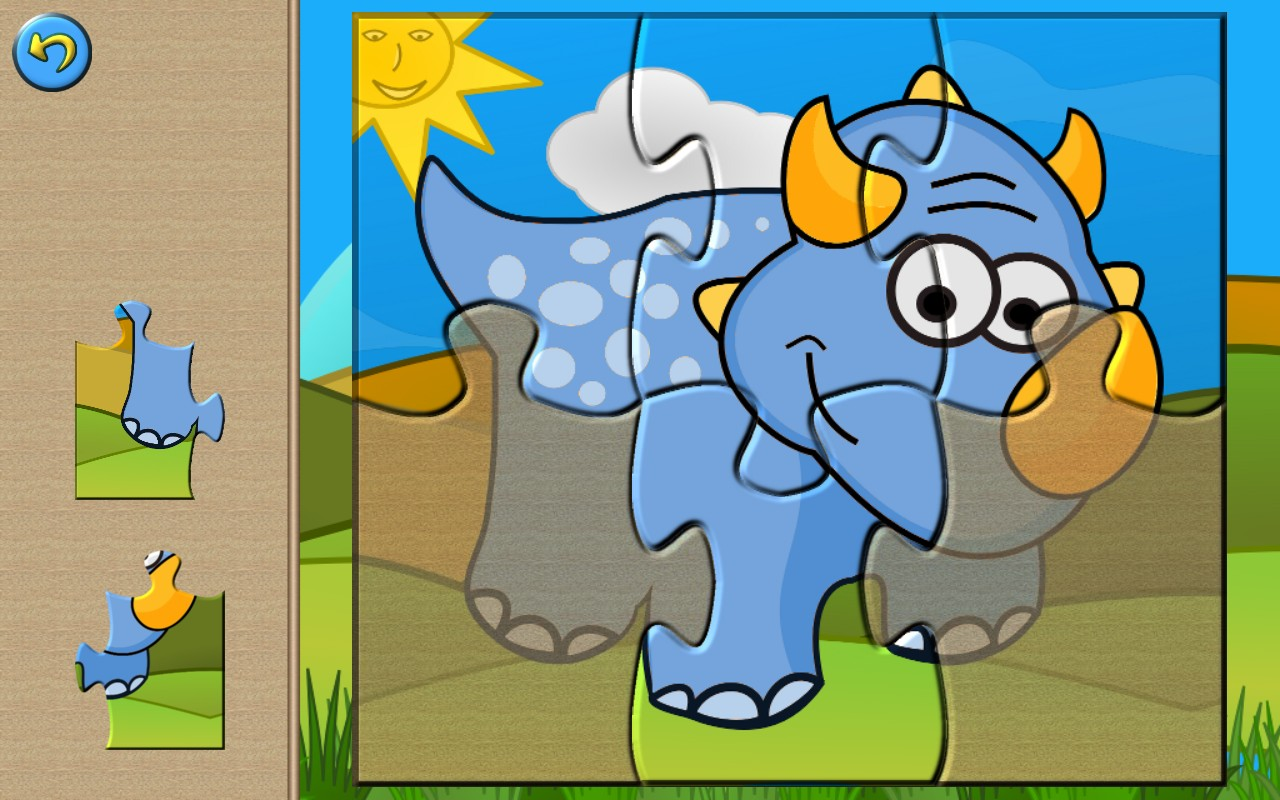
\includegraphics[width=\linewidth]{./Figures/chapter-01/baby-01.jpg}
%		
\includegraphics[width=\linewidth,height=\textheight]{./Figures/chapter-01/baby-02.jpg}
	%	\caption{}
\end{figure}
\end{frame}


%%%%%%%%%%%%%%%%%%%%%%%%%%%%%%%%%%%%%%%%%%%%%%%%%%%%%%
\begin{frame}
\frametitle{Transnational DB Use cases}
\begin{figure}[ht]
	
	\centering
%	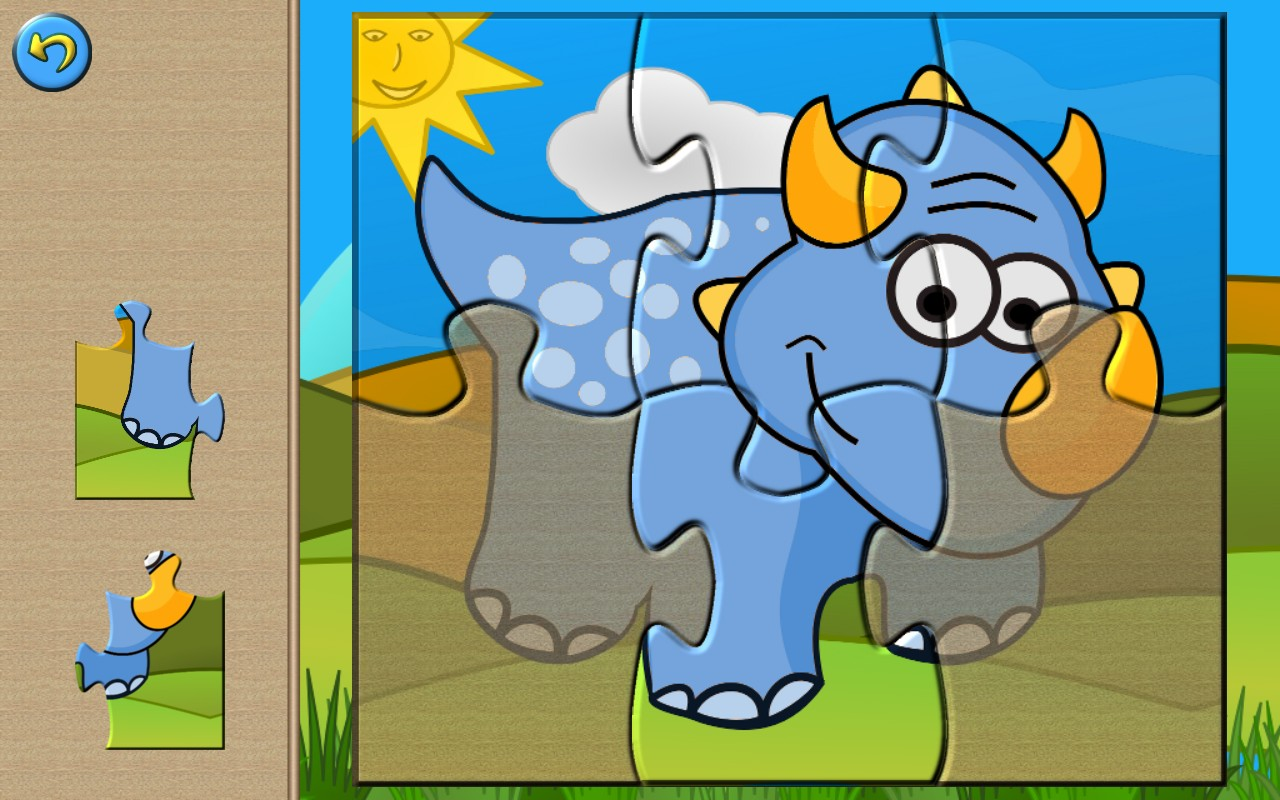
\includegraphics[width=\linewidth]{./Figures/chapter-01/baby-01.jpg}
			
\includegraphics[width=\linewidth]{./Figures/chapter-01/baby-02.jpg}
	%	\caption{}
\end{figure}
\end{frame}


%%%%%%%%%%%%%%%%%%%%%%%%%%%%%%%%%%%%%%%%%%%%%%%%%%%%%%
\begin{frame}
\frametitle{DWH Use cases}
\begin{figure}[ht]
	
	\centering
	
\includegraphics[width=\linewidth,height=.8\textheight]{./Figures/chapter-01/Marvel-03.jpg}
	%	\caption{}
\end{figure}
\end{frame}

%%%%%%%%%%%%%%%%%%%%%%%%%%%%%%%%%%%%%%%%%%%%%%%%%%%%%%
\begin{frame}
\frametitle{DWH Use cases}
\begin{figure}[ht]
	
	\centering
	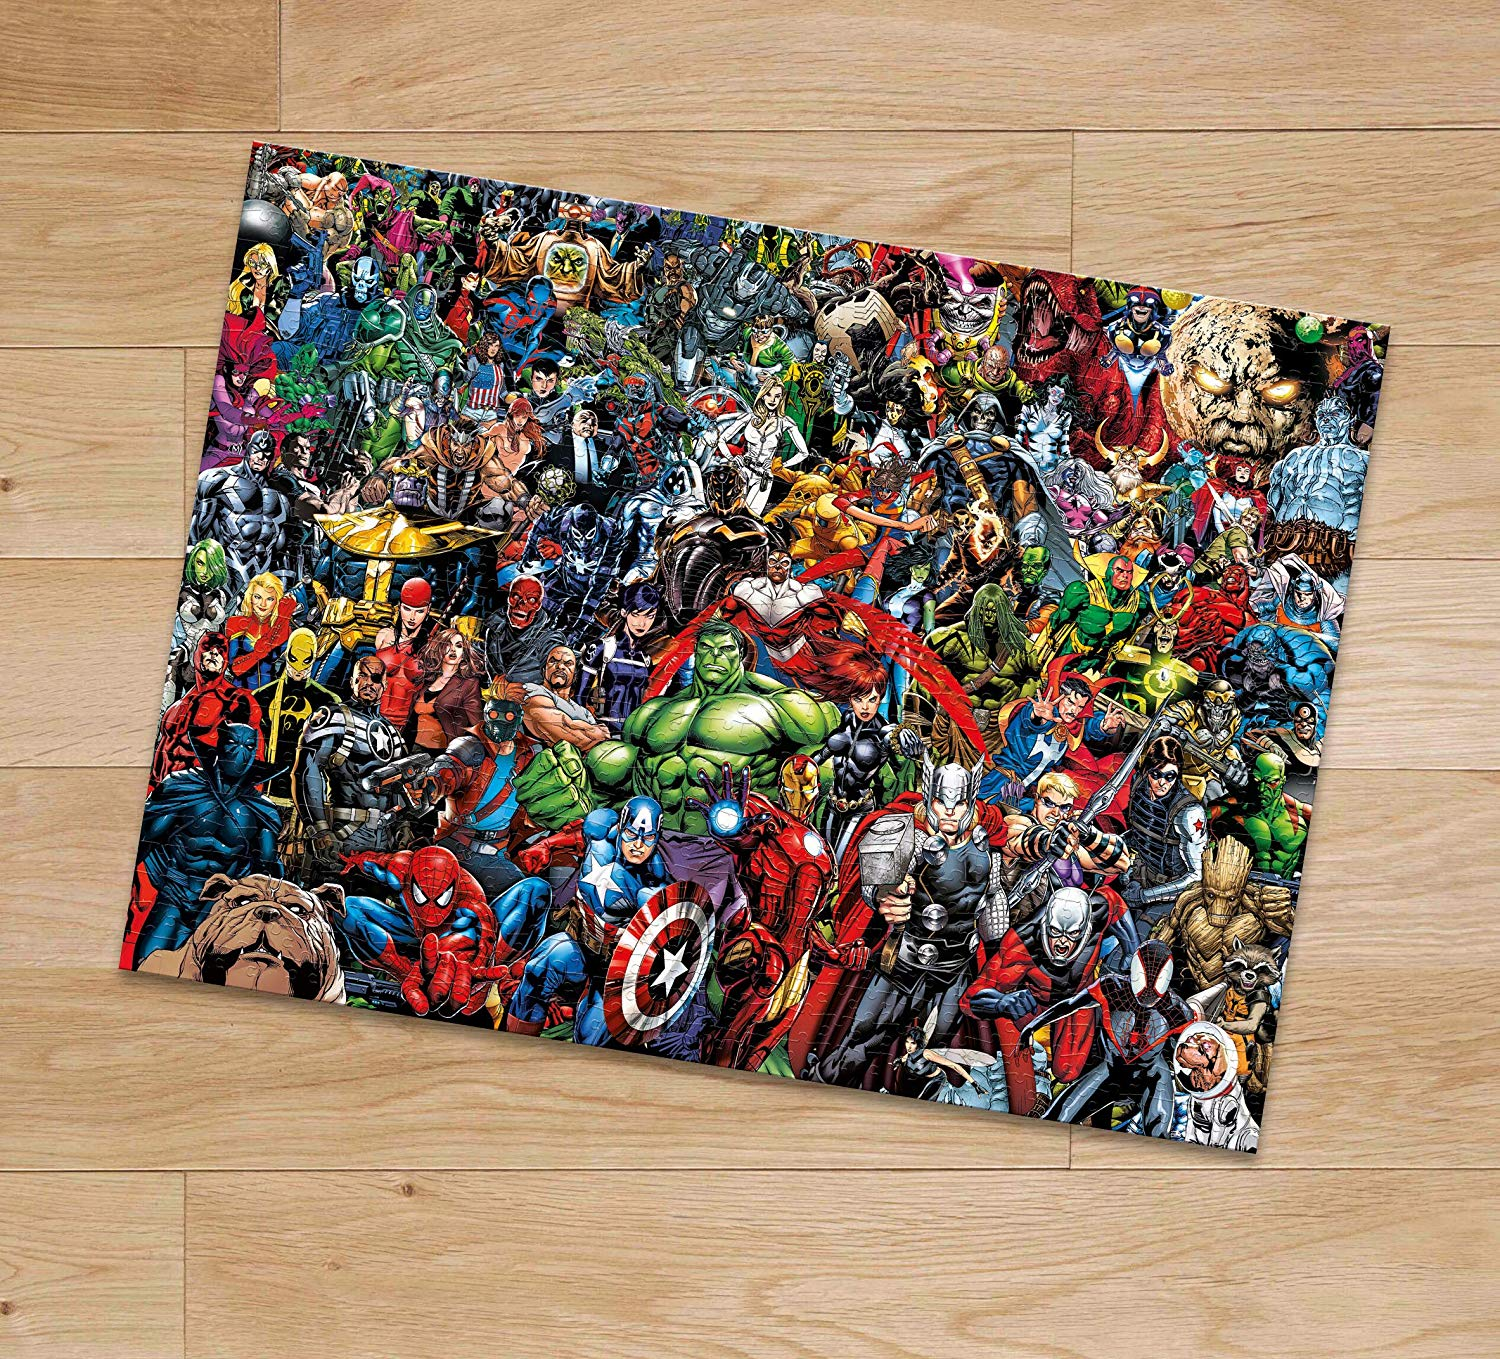
\includegraphics[width=\linewidth,height=.8\textheight]{./Figures/chapter-01/Marvel-02.jpg}
	%	\caption{}
\end{figure}
\end{frame}

%%%%%%%%%%%%%%%%%%%%%%%%%%%%%%%%%%%%%%%%%%%%%%%%%%%%%%
\begin{frame}
\frametitle{DWH Use cases}
\begin{figure}[ht]
	
	\centering
	
\includegraphics[width=\linewidth,height=.8\textheight]{./Figures/chapter-01/Marvel-01.jpg}
	%	\caption{}
\end{figure}
\end{frame}
%%%%%%%%%%%%%%%%%%%%%%%%%%%%%%%%%%%%%%%%%%%%%%%%%%%%%%

User stories Telecom company.

It has a CRM System backend database reporting the sales. vs Another backend database contains the CRM, Telecom signaling data, IN charging system, Billing

Decision is related to sales or CRM. Decision is related to company strategies.
Analytical model checking the fraud which require a CRM data with customer locations from signaling with Billing details from CAR table.
%%%%%%%%%%%%%%%%%%%%%%%%%%%%%%%%%%%%%%%%%%%%%%%%%%%%%%


%%%%%%%%%%%%%%%%%%%%%%%%%%%%%%%%%%%%%%%%%%%%%%%%%%%%%%
managing risk of the project in Transaction vs DWH


%%%%%%%%%%%%%%%%%%%%%%%%%%%%%%%%%%%%%%%%%%%%%%%%%%%%%%


%%%%%%%%%%%%%%%%%%%%%%%%%%%%%%%%%%%%%%%%%%%%%%%%%%%%%%
data model comparison


%%%%%%%%%%%%%%%%%%%%%%%%%%%%%%%%%%%%%%%%%%%%%%%%%%%%%%


\begin{frame}

\frametitle{Cold storage vs Hot storage}

some details about hot vs cold storage,

\end{frame}


%%%%%%%%%%%%%%%%%%%%%%%%%%%%%%%%%%%%%%%%%%%%%%%%%%%%%%

\begin{frame}
\frametitle{DWH Characteristics}

some details about hot vs cold storage,

\end{frame}

%%%%%%%%%%%%%%%%%%%%%%%%%%%%%%%%%%%%%%%%%%%%%%%%%%%%%%

\subsection{Distributed Systems Concepts}
\begin{frame}
\frametitle{\subsecname}
\begin{itemize}[<+->]
	\item Any Big Data solution working based distributed systems.
	\item What is distributed systems in brief?
\end{itemize}
\end{frame}

%%%%%%%%%%%%%%%%%%%%%%%%%%%%%%%%%%%%%%%%%%%%%%%%%%%%%%

\subsection{Hadoop Architecture}
\begin{frame}
\frametitle{\subsecname}
\begin{itemize}[<+->]
	\item Any Big Data solution working based distributed systems.
	\item What is distributed systems in brief?
\end{itemize}
\end{frame}

%%%%%%%%%%%%%%%%%%%%%%%%%%%%%%%%%%%%%%%%%%%%%%%%%%%%%%


\subsubsection{Storage}
\begin{frame}
\frametitle{Storage}
\begin{itemize}[<+->]
	\item Any Big Data solution working based distributed systems.
	\item What is distributed systems in brief?
\end{itemize}
\end{frame}

%%%%%%%%%%%%%%%%%%%%%%%%%%%%%%%%%%%%%%%%%%%%%%%%%%%%%%

\subsubsection{YARN}
\begin{frame}
\frametitle{YARN}
\begin{itemize}[<+->]
	\item Any Big Data solution working based distributed systems.
	\item What is distributed systems in brief?
\end{itemize}
\end{frame}

%%%%%%%%%%%%%%%%%%%%%%%%%%%%%%%%%%%%%%%%%%%%%%%%%%%%%%

\subsubsection{Hadoop I/O}
\begin{frame}
\frametitle{Hadoop I/O}
\begin{itemize}[<+->]
	\item Any Big Data solution working based distributed systems.
	\item What is distributed systems in brief?
\end{itemize}
\end{frame}

%%%%%%%%%%%%%%%%%%%%%%%%%%%%%%%%%%%%%%%%%%%%%%%%%%%%%%

\subsubsection{Processing}
\begin{frame}
\frametitle{Processing}
\begin{itemize}[<+->]
	\item Any Big Data solution working based distributed systems.
	\item What is distributed systems in brief?
\end{itemize}
\end{frame}

%%%%%%%%%%%%%%%%%%%%%%%%%%%%%%%%%%%%%%%%%%%%%%%%%%%%%%

\subsection{Map-Reduce}
\begin{frame}
\frametitle{\subsecname}
\begin{itemize}[<+->]
	\item Any Big Data solution working based distributed systems.
	\item What is distributed systems in brief?
\end{itemize}
\end{frame}

%%%%%%%%%%%%%%%%%%%%%%%%%%%%%%%%%%%%%%%%%%%%%%%%%%%%%%

\subsubsection{Map-Reduce Components}
\begin{frame}
\frametitle{Map-Reduce Components}
\begin{itemize}[<+->]
	\item Any Big Data solution working based distributed systems.
	\item What is distributed systems in brief?
\end{itemize}
\end{frame}

%%%%%%%%%%%%%%%%%%%%%%%%%%%%%%%%%%%%%%%%%%%%%%%%%%%%%%

\subsubsection{Word-Count Example}
\begin{frame}
\frametitle{Word-Count Example}
\begin{itemize}[<+->]
	\item Any Big Data solution working based distributed systems.
	\item What is distributed systems in brief?
\end{itemize}
\end{frame}

%%%%%%%%%%%%%%%%%%%%%%%%%%%%%%%%%%%%%%%%%%%%%%%%%%%%%%

\subsection{Hive}
\begin{frame}
\frametitle{Hive}
\begin{itemize}[<+->]
	\item Any Big Data solution working based distributed systems.
	\item What is distributed systems in brief?
\end{itemize}
\end{frame}
%%%%%%%%%%%%%%%%%%%%%%%%%%%%%%%%%%%%%%%%%%%%%%%%%%%%%%%%%%%%%%%%%%%%%%%%%%%
%%% Local Variables:
%%% mode: latex
%%% TeX-master: "../main"
%%% TeX-engine: xetex
%%% End:

\subsection{Assignment and Homework}